%% uctest.tex 11/3/94
%% Copyright (C) 1988-2004 Daniel Gildea, BBF, Ethan Munson.
%
% This work may be distributed and/or modified under the
% conditions of the LaTeX Project Public License, either version 1.3
% of this license or (at your option) any later version.
% The latest version of this license is in
%   http://www.latex-project.org/lppl.txt
% and version 1.3 or later is part of all distributions of LaTeX
% version 2003/12/01 or later.
%
% This work has the LPPL maintenance status "maintained".
% 
% The Current Maintainer of this work is Daniel Gildea.
%
% 2007/08/01
% LaTeX Package "ucr" is modified from LaTeX package "ucthesis."
% This modification is therefore under to the conditions of 
% the LaTeX Project Public License.
% Its formality is suitable for the dissertation of Universty of
% California, Riverside.
% This test document is for the convenience of all students of
% Universty of California, Riverside.
% Contact Charles Yang at chcyang@yahoo.com if you like.
% Charles Yang has nothing to do with the original author's sarcasm.
%
% \documentclass[11pt]{ucthesis}
% \documentclass[11pt]{ucr}
\documentclass[oneside,final, letterpaper]{ucr}
\begin{document}

% Declarations for Front Matter

\title{The Title of Your Thesis Goes Here}
\author{Clarity Laska Shimoniak}
\degreemonth{March}
\degreeyear{2024}
\degree{Master of Science}
\chair{Dr. Philip Brisk}
\othermembers{Dr. Daniel Wong\\
Dr. Karen Smith}
\numberofmembers{3}
\field{Computer Engineering}
\campus{Riverside}

\maketitle
\copyrightpage{}
\approvalpage{}

\degreesemester{Fall}

\begin{frontmatter}

\begin{acknowledgements}
I am grateful to my advisor, without whose help, I would not have been here.
\end{acknowledgements}

\begin{dedication}
\null\vfil
{\large
\begin{center}
To my parents for all the support.
\end{center}}
\vfil\null
\end{dedication}

\begin{abstract}
% Abstract should be double-spaced and limited to 350 words or 2,450 characters.
Both FPGAs and RDMA have seen increasing adoption in datacenters as a means of achieving the parallelism and responsiveness needed in modern applications. We propose a novel database architecture built around a distributed FPGA cluster with RDMA as its interconnect in order to implement high-performance, in-memory key-value store based on the B-Link tree.
\end{abstract}


\tableofcontents
\listoffigures
\listoftables
\end{frontmatter}

% \part{First Part}


\section{Introduction}

\subsection{FPGA}

Field-Programmable Gate Arrays

that have seen increasing adoption with decreasing costs.

One application that FPGAs are uniquely for is networking, as the dataflow programming model aligns well with the way that streams of data are processed in high throughput networking situations. FPGAs have seen increasing deployment in datacenters as a means to improve the underlying datacenter infrastructure \todocite, rather than simply as accelerators as GPUs are.


\subsection{RDMA}

Remote Direct Memory Access (RDMA) is an extension to the concept of direct memory access (DMA), which a system's memory to be accessed without the involvement of its CPU. RDMA is a standard allowing for such transactions to take place over a network rather than a local like like PCIe. Compared to traditional networking protocols, RDMA is significantly faster, moving the bottleneck of distributed systems out of the networking portion and into processing portion \cite{binnig-vldb-2016}.

RDMA has also seen widespread datacenter adoption, though primarily on CPU-based systems that use specialized network interface cards (NICs) to handle RDMA operations.

\citet{star} has shown the viability of FPGAs as network accelerators, but \citeauthor{star} use them to implement custom a NIC rather than as part of an application \cite{star}.

RDMA operations can be either one-sided or two-sided. One-sided operations access memory at a specific location on the remote node. These are lightweight and simple to implement, but are more difficult for applications to use. Two-sided operations  \cite{base}.

For CPU systems, there is a tradeoff between the two types of operations. Using an FPGA


\subsection{B-Link Tree}

B-Link trees are an extension to B+ trees proposed by \citeauthor{b-link} to support concurrency. Like B+ trees, they are self-balancing data structures with an adjustable fan-out factor that store all data at leaf nodes. B-Link trees introduce additional linkages between nodes and ensure that no more than three nodes are locked at a time-per transaction \cite{b-link}.
 %usually intro
\chapter{Chapter 2 Title}


\section{Memory Layout}

The primary challenge of converting the design proposed by \citeauthor{base} from CPU to FPGA is that all memory must be managed manually. There is no operating system or standard library to dynamically allocate memory or handle virtual addressing. This makes it desirable for addresses of nodes within a tree to change as little as possible, as without an internal address translation layer, any movement of a node within a cluster would require that address change to be broadcast to all other nodes in the cluster, unnecessarily consuming channel bandwidth.

\newcommand{\clusternode}[1]{
	% Cluster Boundary
	\draw ({(#1)*6}, 0) ++(-2.75, 0.5) rectangle ++(5.5, -3);
	% Tree Nodes
	\node[tree] at ({(#1)*6}, 0) (n#1 00) {};
	% Rows
	\foreach \r [
		evaluate = \r as \w using int(3^\r),
		evaluate = \r as \wl using int(3^\r-1)
	] in {1,...,2} {
		% Columns
		\foreach \c [
			evaluate = \c as \i using int((\w-1)/2 + \c-1),
			evaluate = \c as \pr using int(\r-1),
			evaluate = \c as \pc using int(\c/3),
			evaluate = \c as \cl using int(\c-1)
		] in {0,...,\wl} {
			\node[tree] (n#1 \r\c)
				at ({(#1)*6 + (\c-int(\w/2)) / (\w/5)}, -\r) {};
			\draw[->] (n#1 \pr\pc) -- (n#1 \r\c);
			\ifthenelse{\c=0}{}{
				\draw[->] (n#1 \r\cl) -- (n#1 \r\c);
			}
		}
	}
}

\begin{figure}
\centering
\begin{tikzpicture}[
	scale=0.7,
	tree/.style={draw,circle,inner sep=0.5mm}
]
	\clusternode{0}
	\clusternode{1}
	\draw[->] (n0 00) -- (n1 00);
	\draw[->] (n0 12) -- (n1 10);
	\draw[->] (n0 28) -- (n1 20);
\end{tikzpicture}
\caption{Linkages Between Nodes in the Cluster}
\end{figure}

\citeauthor{base} also propose a fine-grained distribution. The downside of this approach for an FPGA system is that increasing linkage between trees and thus the number of nodes that cannot be moved.

\section{Experiment}

\begin{figure}
	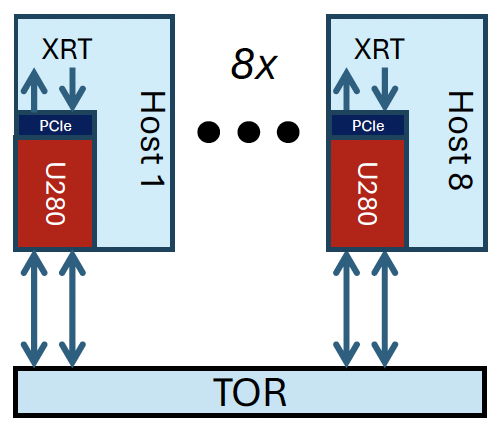
\includegraphics[width=2in]{oct-arch.jpg}
	\caption{Cluster Architecture}
	\label{oct-arch}
\end{figure}

The database was implemented on a cluster of 8 nodes that share a single network switch as shown in figure \ref{oct-arch}. Each node has a Xilinx Alveo U280 PCIe card, containing a XCU280 FPGA and $\SI{8}{\giga\byte}$ of high-bandwidth memory (HBM). Each node is connected to the switch with a $\SI{100}{\giga\bit}$ NIC.

\section{Conclusions}

Conclusions go here




\nocite{*}
% \singlespacing
% \bibliographystyle{alpha}
\bibliographystyle{plain}
\bibliography{bibfile}

../common/appendix.tex


\end{document}
